\chapter{Evaluation results}
This appendix will give an overview of the raw results gathered by the evaluations performed on the different prototypes.
\section{Capacitive chair posture recognition}
\label{ch:app_capchair_eval}
This section provides raw data of the first posture recognition test performed using the capacitive chair. 
\subsection{Evaluation setup}
Short study with 10 participants. Three poses and a non-pose:
\begin{itemize}
\item Sitting upright
\item Sitting hunched
\item Slouching on chair
\item Close to chair - disturber
\end{itemize}

The persons were given a short introduction, the different postures were displayed, and finally the persons were asked to perform the postures in order. When testing “close-to-chair” the subjects were asked to rattle at the chair, stand close, move it around and thus disturb the potential sensor readings. Each class was tested for 10 seconds, collecting 200 samples. 

\subsection{Raw results}
\begin{table}[htbp]
  \centering
  \caption{Percentage of correctly classified postures using manually set classifier}
    \begin{tabularx}{\linewidth}{XXXXXXXXXXXX}
    \toprule
          & S1    & S2    & S3    & S4    & S5    & S6    & S7    & S8    & S9    & S10   & Avg \\
    \midrule
    Upright & 100   & 100   & 100   & 100   & 100   & 100   & 100   & 100   & 100   & 100   & 100 \\
    Hunched & 100   & 100   & 100   & 100   & 86    & 100   & 100   & 100   & 100   & 100   & 98,6 \\
    Slouch & 100   & 100   & 100   & 100   & 100   & 100   & 100   & 100   & 55    & 100   & 95,5 \\
    Disturber & 100   & 100   & 100   & 100   & 100   & 100   & 100   & 100   & 100   & 100   & 100 \\
    \bottomrule
    \end{tabularx}%
  \label{tab:app_eval_chair_raw1}%
\end{table}%
\subsection{Postures}
\begin{figure}[ht]
\centering
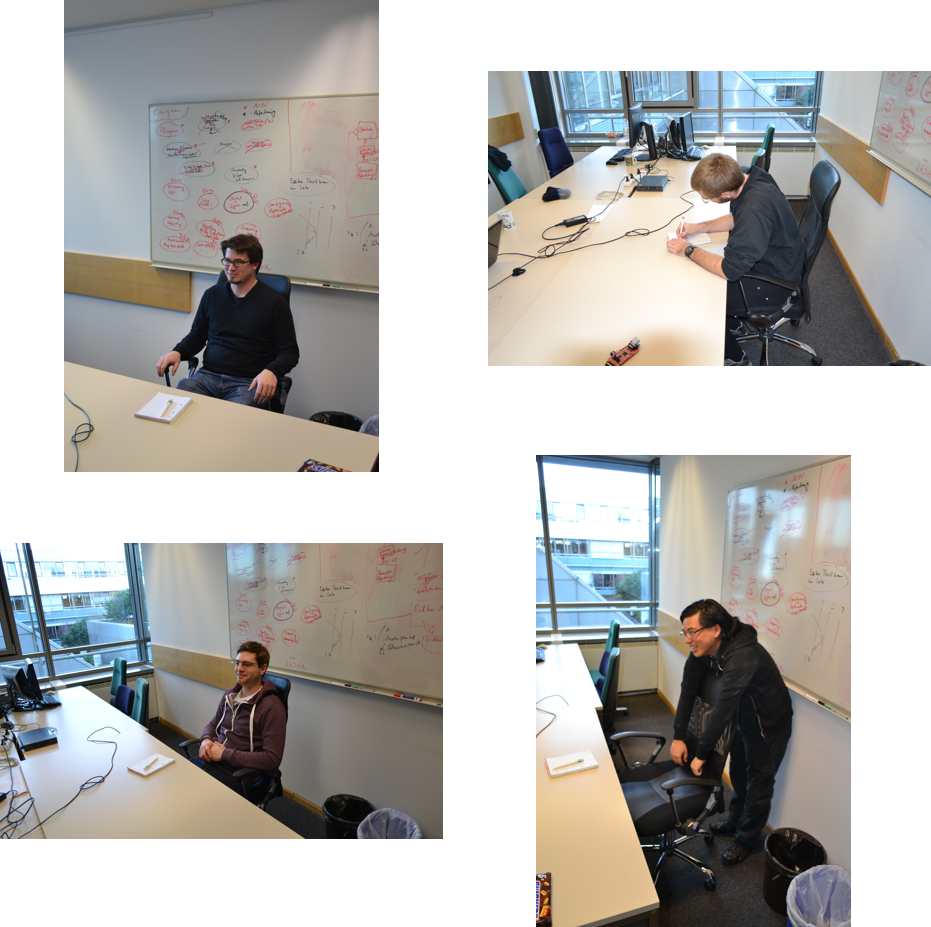
\includegraphics[width=0.8\textwidth]{images/app_eval_chair1}
\caption{\emph{Top left} upright posture. \emph{Top right} hunched posture. \emph{Bottom left} slouched posture. \emph{Bottom right} disturber posture}
\label{fig:disc_unob_elec}
\end{figure}

\section{Capacitive Chair - working situation recognition}
\begin{figure}[ht]
\centering
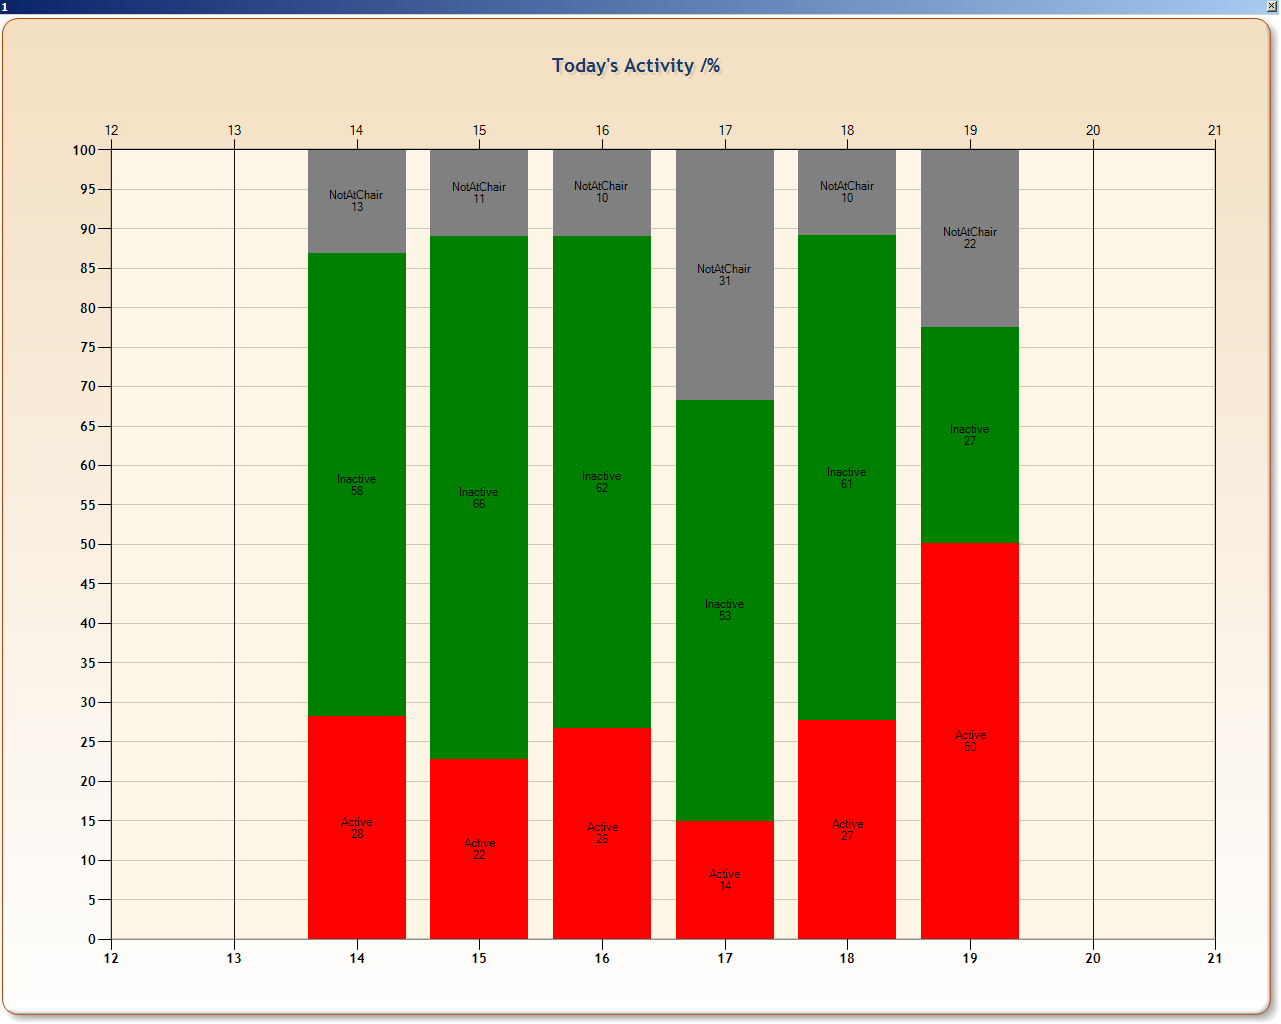
\includegraphics[width=0.6\textwidth]{images/workact_day1}
\caption{Work activity day 1}
\label{fig:workact_day1}
\end{figure}

\begin{figure}[ht]
\centering
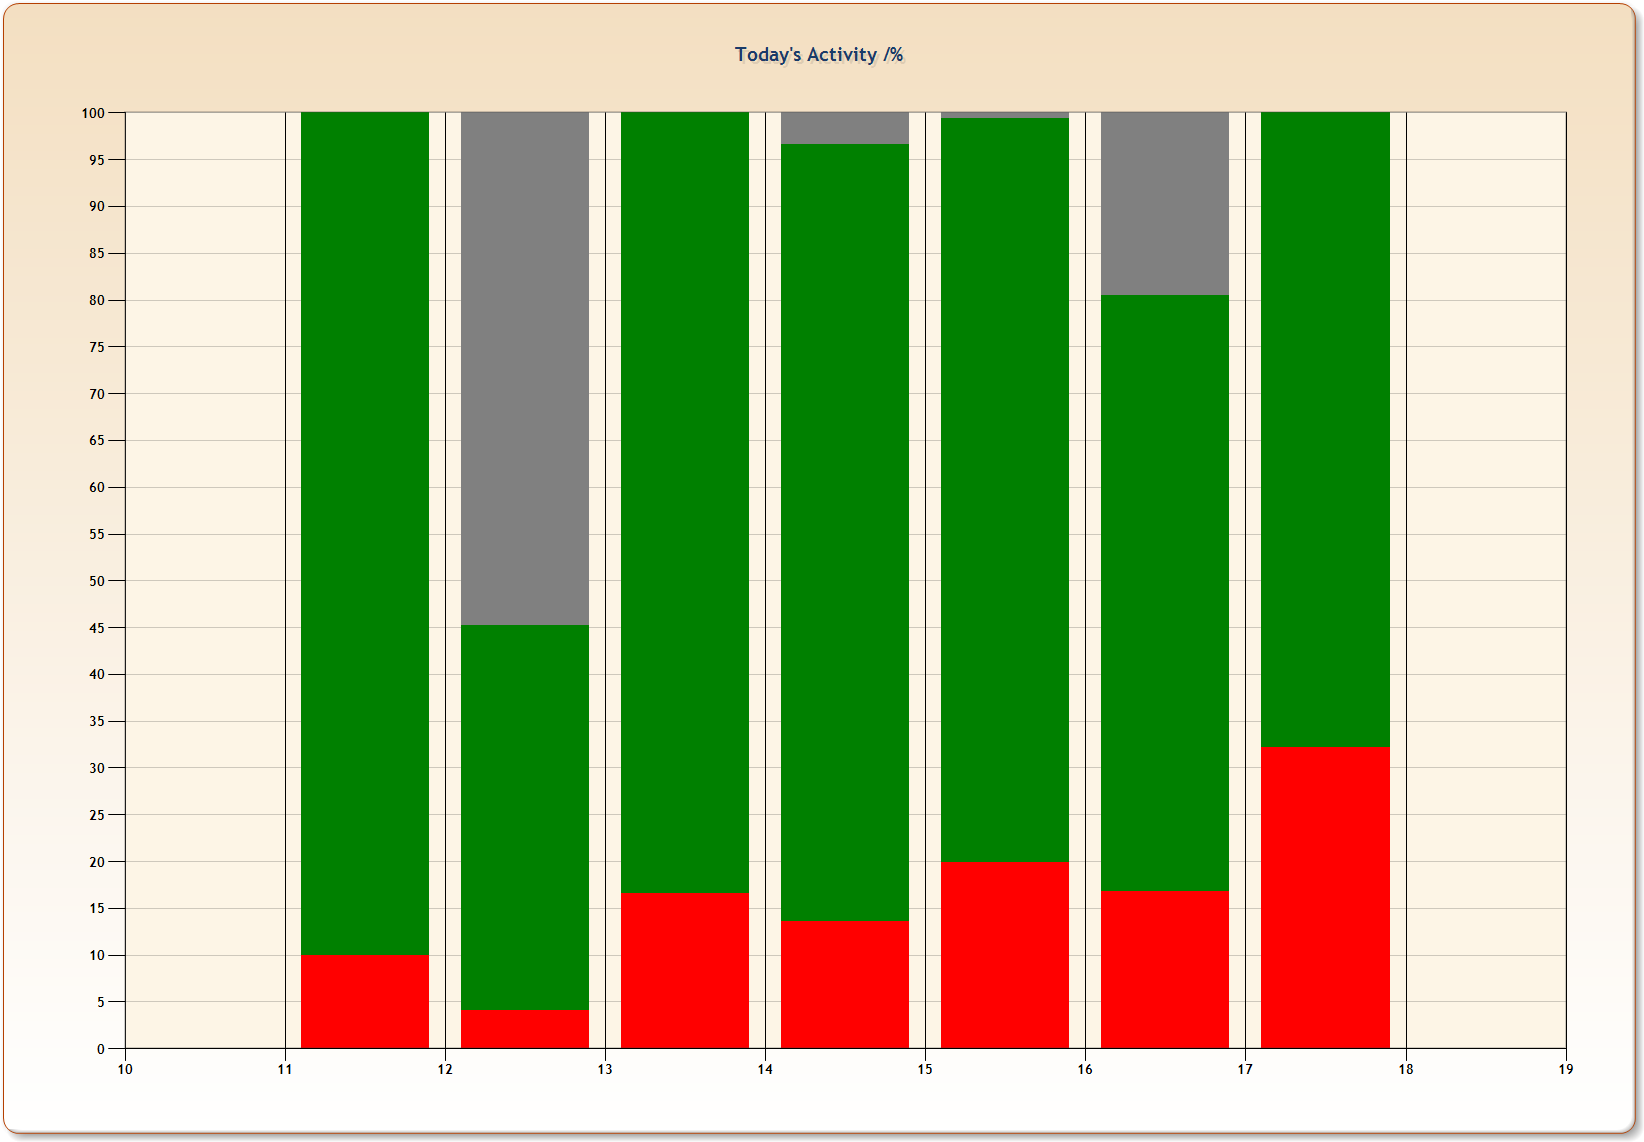
\includegraphics[width=0.6\textwidth]{images/workact_day2}
\caption{Work activity day 2}
\label{fig:workact_day2}
\end{figure}

\begin{figure}[ht]
\centering
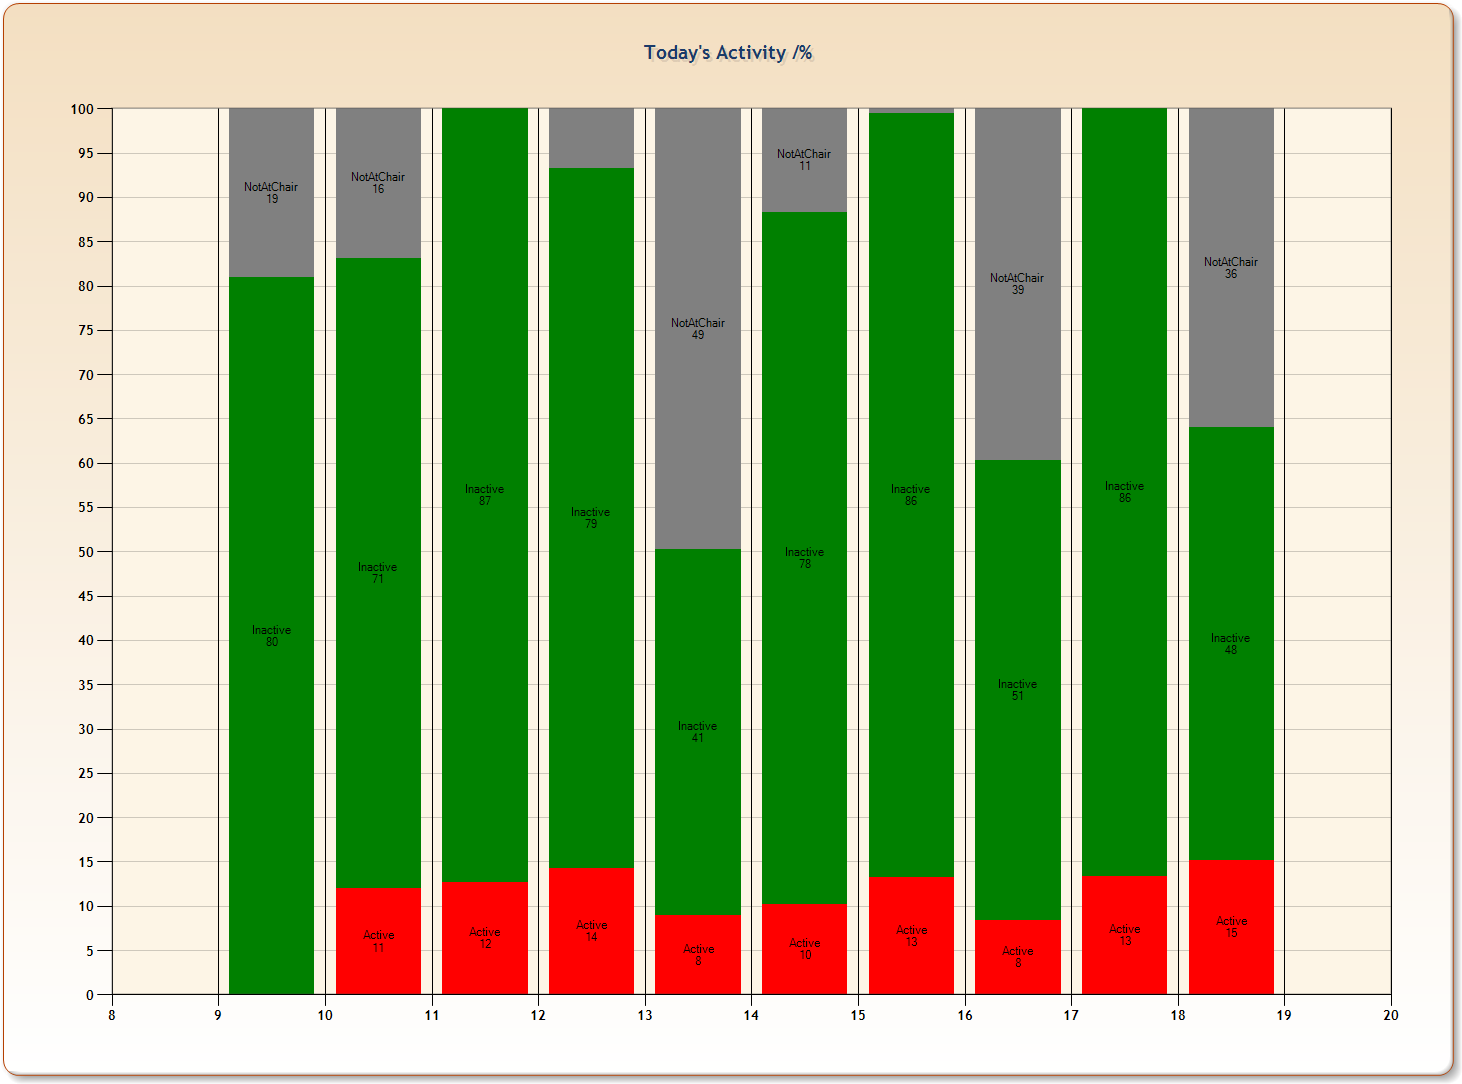
\includegraphics[width=0.6\textwidth]{images/workact_day3}
\caption{Work activity day 3}
\label{fig:workact_day3}
\end{figure}


\section{CapTap evaluation}
\subsection{Questionnaire}
\begin{itemize}
\item G1 Experience with touch screen systems (none = 1, daily usage = 10)
\item G2 Experience with gesture recognition systems (none = 1, daily usage = 10)
\item Q1 Do you agree that the required tasks were easy and precise to perform? (Not agree = 1, Strong agree = 10)
\item Q2 Was the CapTap to be intuitive in its usage? (Not agree = 1, Strong agree = 10)
\item Q3 I could control the different layers in the painter application? (Not agree = 1, Strong agree = 10)
\item Q4 I could control the different interactions in the test run? (Not agree = 1, Strong agree = 10)
\item Q5 Do you prefer finger swipes or hand swipes?
(Finger swipe = 1, Hand swipe = 10)
\item Q6Do you prefer finger taps or knuckle knocks? (Finger taps = 1, Knuckle knocks = 10)
\item Q7 The CapTap should support more than three interaction layers? (Not agree = 1, Strong agree = 10)
\item Q8 Do you agree that CapTap is an interesting form of interaction device? (Not agree = 1, Strong agree = 10)
\item Q9 Would you consider using an input device like CapTap for a longer period of time? (Not at all = 1, I would like to use it = 10)
\item Q10 What did you particularly like about the CapTap?
\item Q11 What did you particularly dislike about the CapTap?
\end{itemize}

\subsection{Raw results}
The table denotes the results of the different touch points as explained in the descriptive section. The T's refer to the times of the three different interaction speed runs.

\begin{landscape}
\begin{table}[htbp]
  \footnotesize
  \centering
  \caption{CapTap evaluation raw results}
    \begin{tabular}{rrrrrrrrrrrrrrrrrrrrrrrrr}
    \toprule
    Subject & 1     & 1D    & 2     & 2D    & 3     & 3D    & 4     & 4D    & 5     & 5D    & 6     & 6D    & 7     & 8     & 9     & 10    & 11    & 12    & 13    & 14    & 15    & T1    & T2    & T3 \\
    \midrule
    S1    & 3     & 3     & 3     & 3     & 3     & 3     & 1     & 3     & 2     & 0     & 1     & 2     & 3     & 3     & 3     & 3     & 3     & 3     & 3     & 3     & 3     & 45,38 & 41,57 & 33,94 \\
    S2    & 3     & 3     & 3     & 3     & 3     & 3     & 3     & 3     & 3     & 3     & 3     & 3     & 3     & 3     & 3     & 3     & 3     & 3     & 3     & 3     & 3     & 43,12 & 41,83 & 36,94 \\
    S3    & 3     & 2     & 3     & 3     & 3     & 3     & 3     & 2     & 2     & 2     & 2     & 2     & 2     & 3     & 0     & 3     & 3     & 3     & 1     & 3     & 3     & 51,38 & 34,42 & 31,33 \\
    S4    & 3     & 3     & 3     & 3     & 3     & 3     & 3     & 3     & 3     & 3     & 3     & 3     & 3     & 3     & 3     & 3     & 3     & 3     & 3     & 3     & 3     & 27,28 & 34,17 & 24,29 \\
    S5    & 3     & 2     & 2     & 3     & 3     & 3     & 3     & 1     & 3     & 3     & 3     & 1     & 2     & 3     & 3     & 3     & 3     & 3     & 2     & 3     & 2     & 34,66 & 48,11 & 45,35 \\
    S6    & 3     & 3     & 3     & 3     & 3     & 3     & 3     & 3     & 3     & 2     & 2     & 1     & 3     & 3     & 3     & 3     & 3     & 3     & 1     & 3     & 1     & 39,28 & 42,62 & 47,72 \\
    S7    & 3     & 3     & 3     & 3     & 3     & 3     & 3     & 3     & 3     & 2     & 3     & 3     & 0     & 1     & 3     & 1     & 3     & 3     & 1     & 3     & 1     & 40,87 & 33,56 & 25,95 \\
    S8    & 3     & 3     & 3     & 3     & 3     & 3     & 2     & 0     & 1     & 1     & 3     & 0     & 3     & 3     & 3     & 3     & 3     & 3     & 3     & 3     & 1     & 47,14 & 37,43 & 32,72 \\
    S9    & 3     & 3     & 3     & 3     & 3     & 2     & 2     & 3     & 1     & 0     & 2     & 2     & 0     & 3     & 0     & 3     & 3     & 3     & 1     & 3     & 2     & 39,71 & 33,78 & 26,63 \\
    S10   & 3     & 3     & 3     & 3     & 3     & 3     & 2     & 0     & 3     & 0     & 2     & 0     & 3     & 3     & 1     & 3     & 3     & 3     & 2     & 1     & 1     & 32,35 & 32,2  & 29,31 \\
    Ergebnis & 30    & 28    & 29    & 30    & 30    & 29    & 25    & 21    & 24    & 16    & 24    & 17    & 22    & 28    & 22    & 28    & 30    & 30    & 20    & 28    & 20    & 40,117 & 37,969 & 33,418 \\
    \bottomrule
    \end{tabular}%
  \label{tab:app_eval_captap_raw_quant}%
\end{table}%
\end{landscape}
\begin{landscape}
% Table generated by Excel2LaTeX from sheet 'Tabelle3'
\begin{table}[htbp]
  \footnotesize
  \centering
  \caption{CapTap questionnaire results}
    \begin{tabular}{rrrrrrrrrrrrm{4.5cm}m{4.5cm}}
    \toprule
    Subject & G1    & G2    & Q1    & Q2    & Q3    & Q4    & Q5    & Q6    & Q7    & Q8    & Q9    & Q10   & Q11 \\
    \midrule
    S1    & 10    & 5     & 6     & 9     & 9     & 8     & 8     & 1     & 6     & 10    & 9     & unsichtbare Sensorik im vertrauten Möbelstück, Gesten über Tisch & Präzision nicht gut genug \\
    S2    & 10    & 9     & 6     & 8     & 6     & 8     & 7     & 3     & 3     & 7     & 6     & Nice idea of embedding interaction into everyday furniture & area is too large, interaction is exhausting, demonstrator table not suitable \\
    S3    & 10    & 4     & 10    & 10    & 5     & 10    & 10    & 1     & 1     & 10    & 7     & tactility, intuitive and invisible & some areas hard to reach when sitting in front \\
    S4    & 10    & 8     & 8     & 9     & 8     & 9     & 2     & 1     & 4     & 10    & 8     &       & some errors in interaction \\
    S5    & 10    & 3     & 10    & 8     & 8     & 8     & 2     & 1     & 6     & 9     & 8     & touchpad like control on table & knocking, interaction disturbed by knee \\
    S6    & 10    & 8     & 8     & 9     & 7     & 8     & 3     & 3     & 3     & 9     & 8     & unobtrusive integration in furniture, intuitive interaction & delay in recognition \\
    S7    & 10    & 10    & 10    & 10    & 5     & 10    & 3     & 2     & 5     & 10    & 8     & Eingaben mit und ohne Kontakt, Auswahl über Tap intuitiv, Schnelle Eingewöhnung in Layer mit Farben & Beine werden erkannt, große Interaktionsarea, Verzerrungen im Zeichenprogramm \\
    S8    & 10    & 3     & 7     & 8     & 7     & 9     & 2     & 2     & 1     & 7     & 4     & ease of use, low learning curve, big variety of input modalities & interaction less precise in some areas \\
    S9    & 10    & 3     & 8     & 9     & 4     & 7     & 7     & 10    & 3     & 9     & 3     & knockin on heaven's door & tap didn't work - required more than one tap to recognize \\
    S10   & 4     & 7     & 8     & 9     & 7     & 9     & 2     & 2     & 7     & 10    & 8     & different interaction possibilities & detection of knees, difficulty to stay in layer \\
    Ergebnis & 9,4   & 6     & 8,1   & 8,9   & 6,6   & 8,6   & 4,6   & 2,6   & 3,9   & 9,1   & 6,9   &       &  \\
    \bottomrule
    \end{tabular}%
  \label{tab:app_eval_captap_raw_quest}%
\end{table}%
\end{landscape}

\section{Active Armrest evaluation results}
\subsection{Questionnaire}
\begin{itemize}
\item G1 Experience with touch screen systems (none = 1, daily usage = 10)
\item G2 Experience with gesture recognition systems (none = 1, daily usage = 10)
\item Q1 Do you agree that the required tasks were easy and precise to perform? (Not agree = 1, Strong agree = 10)
\item Q2 Was the Interactive Armrest to be intuitive in its usage? (Not agree = 1, Strong agree = 10)
\item Q3 Do you prefer multi-touch or basic gestures?
(Multi-touch = 1, Basic gesture = 10)
\item Q4 Is the Interactive Armrest with Multi-touch easy to use? (Not Agree = 1, Strong Agree = 10)
\item Q5 Is the Interactive Armrest with basic gestures easy to use? (Not Agree = 1, Strong Agree = 10)
\item Q6 Do you agree that the Interactive Armrest is an interesting form of interaction device? (Not agree = 1, Strong agree = 10)
\item Q7 Would you consider using an input device like the Interactive Armrest for a longer period of time? (Not at all = 1, I would like to use it = 10)
\item Q8 What did you particularly like about the Interactive Armrest?
\item Q9 What did you particularly dislike about the Interactive Armrest?
\end{itemize}

\section{CapFloor @ EvAAL 2011}
\begin{figure}[ht]
\centering
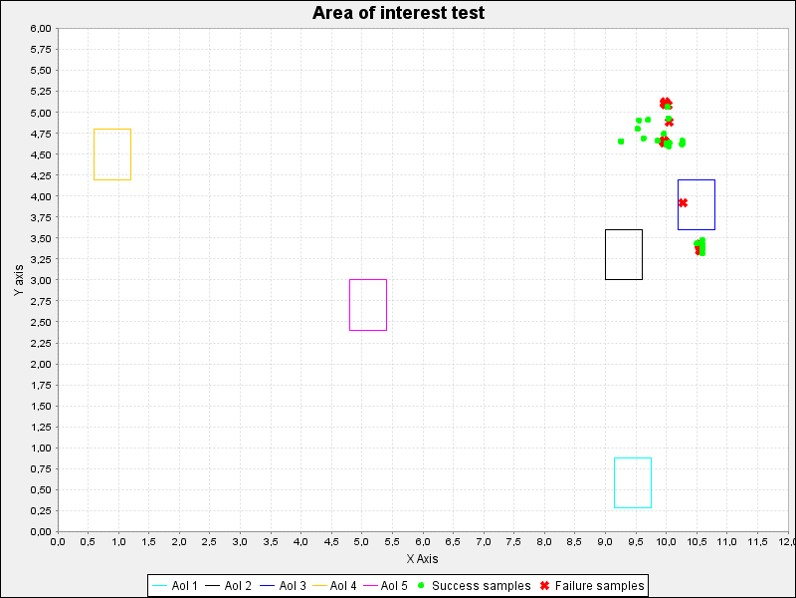
\includegraphics[width=0.6\textwidth]{images/eval_evaal_aoi}
\caption{Recognition rate of CapFloor on selected areas of interest}
\label{fig:eval_evaal_aoi}
\end{figure}

\begin{table}[htbp]
  \centering
  \caption{Best case scores of CapFloor @ EvAAL 2011}
    \begin{tabular}{rrr}
    \toprule
          & \multicolumn{2}{c}{Availability} \\
    \midrule
          & Run 1 & Run 2 \\
    Number of wrong samples & 210   & 258 \\
    Number of total received samples & 328   & 437 \\
    T     & 0.3597561 & 0.40961098 \\
    Accuracy Score & 3.59756098 & 4.09610984 \\
        \midrule
          & \multicolumn{2}{c}{Accuracy} \\
    Available samples & 358   & 437 \\
    Expected samples & 452   & 452 \\
    Availability & 0.7920354 & 0.96681416 \\
    Availability score & 7.92035398 & 9.66814159 \\
    \bottomrule
    \end{tabular}%
  \label{tab:evalres_capfloor}%
\end{table}%

\section{Smart Bed sleep phase recognition results}
\begin{figure}[ht]
\centering
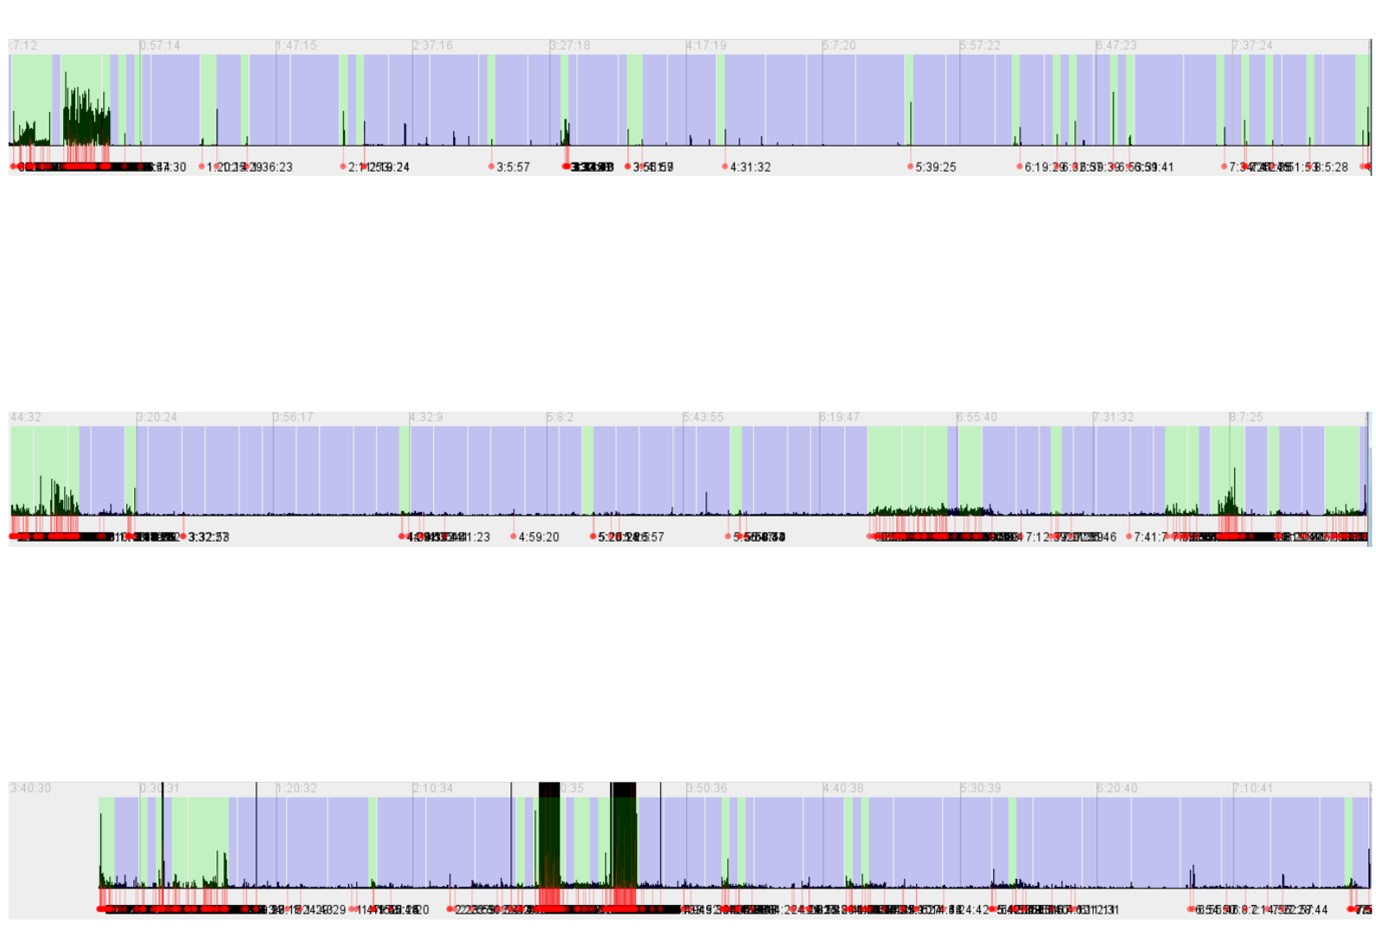
\includegraphics[width=1.0\textwidth]{images/eval_sleep_phase}
\caption{Recognition of sleep phases over three nights}
\label{fig:eval_sleep_phase}
\end{figure}



